\chapter{Implementation, Integration and Test plan}

\section{Overview}

This section outlines the processes of implementation, integration, and testing for the Students\&Companies
(S\&C) platform, describing how its key functionalities were developed and validated to ensure
reliability and effectiveness.

The chapter is divided into three main parts:

\begin{enumerate}
    \item Feature Identification: This part focuses on the platform's key functionalities, derived from
    primary use cases, and highlights the microservices that support them. 
    \item Component Integration and Testing: This section describes the integration of microservices
    to test features, using a thread-based strategy that mirrors real-world scenarios.
    \item System Testing: Here, the focus shifts to testing the platform as a whole, ensuring that
    all components work together seamlessly to deliver a complete and robust system.
\end{enumerate}

The platform was designed with a microservices-based architecture, enabling the division
of functionalities into modular components. During implementation, each microservice was
developed to address a specific aspect of the system, such as recommendation, selection
process management, or feedback handling. However, the testing strategy was designed to go
beyond validating individual components, ensuring that the overall system functionalities
meet the required specifications.

The testing process was executed in three phases:
\begin{enumerate}
    \item Unit Testing: In the first phase, unit tests were performed on individual microservices to ensure
    that each component functions correctly in isolation. This phase focused on verifying the internal
    logic and functionality of each microservice, ensuring a solid foundation for the system.
    \item Feature Integration Testing: The next phase involved integration testing based on the
    platform's key features. Microservices were integrated to test specific use cases, such as the
    matching process between students and companies, ensuring that they worked together as intended.
    A thread-based strategy was used to test these features incrementally, starting from simple
    interactions and gradually integrating more complex functionalities.
    \item System Testing: In the final phase, comprehensive system tests were performed to validate
    the entire platform. This stage involved testing the system as a whole, ensuring that all
    microservices and integrated features functioned cohesively and met the overall functional requirement
\end{enumerate}    
 
By combining unit tests, feature-based integration tests, and comprehensive system testing,
this approach provides a robust framework to identify and resolve issues progressively.
This ensures that the final system is both scalable and reliable, meeting the diverse needs of its users.

\newpage
\section{Implementation Plan}
\subsection{Features Identification}

For the development of the Students\&Companies (S\&C) platform, several key features have been
identified, each representing a core functionality that directly supports user interactions
and business processes. The order in which these features are listed reflects the sequence
in which they will be implemented and tested. Each feature is a logical component of the system,
providing specific, user-visible functionalities that contribute to the overall experience and
effectiveness of the platform.

\subsubsection{Profile Creation Features}

The profile creation feature is available for students, companies, and universities.
For students and companies, the feature is more detailed compared to universities. 

For students, the functionality includes the ability to initially register on the
platform, add information to their profile, and upload photographs and documents.  
For companies, they must be able to upload information and photographs to their
profiles and create pages for internships, where they can also upload relevant information,
photos, and documents.  
For universities, the profile functionality is simpler; they only need to upload basic information.

Furthermore, in the meantime, the Statistical Analysis Tool collects data
from students and companies, both from their profiles and their actions.

\subsubsection{Selection Process Management Features}

The selection process management feature consists of several stages.

Initially,
the student browses company profiles and views their internship opportunities. When the student
finds an interesting internship, they apply to start the selection process. At this point, the
company reviews the student's profile and decides whether to accept them into the selection process.
If the decision is positive, a notification is sent to the student, informing them of the acceptance.
This new association is then saved.

The platform also supports managing the selection process by enabling questionnaires through the
system and providing the option for online interviews.

\subsubsection{Communication Features}

The communication feature is designed to facilitate interaction between students and companies
throughout the internship. This feature includes two main components.

The first is the official
internship page, a dedicated space where both parties can interact with distinct permissions.
Companies have the ability to post announcements, while students can engage by commenting on
these posts. 

The second component is a direct chat, which functions as a private messaging system between
the student and the company. This allows for streamlined discussions and the exchange of
internship-related information.

Notifications are sent to users to highlight important events, such as new official
announcements, incoming chat messages, or the conclusion of the internship. All data
related to these communications and the internship itself is securely stored in the database.

\subsubsection{Overview of the features: feedback and complaints collection, recommendation,
and complaint report}

For clarity, here is an overview of the features: feedback and complaints collection,
recommendation, and complaint report. These features will be analyzed in detail later on.

The static analysis tool collects preliminary data from student profiles, company profiles,
as well as data during the selection process and the internship (see UC 4, 5, 6, and 7).
The feedback and complaints microservice periodically requests feedback from both students
and companies, both during the selection process and throughout the internship, and records
any complaints (see UC 10).

The static analysis tool then receives and processes this data, sending the relevant
information to the recommendation microservice for recommendations and to the feedback
and complaints microservice for complaint reports (see UC 11). The recommendation
microservice produces the actual recommendations (see UC 12), while the feedback
and complaints microservice generates the complaint report (see UC 13).

\subsubsection{Feedback and Complaints Collection Features}
\subsubsection{Providing Recommendations Features}
\subsubsection{Complaints Report Generation Features}

\subsection{Components Integration and Testing}

In the integration testing phase of the Students\&Companies (S\&C) platform, a hread-based strategy
was chosen to ensure a systematic and realistic evaluation of the system. This approach focuses on
testing complete end-to-end flows, or "threads," that represent specific use cases, such as matching
students with internships or managing the selection process. 

The thread-based strategy was selected because it allows the system to be tested in a way that
closely mirrors real-world usage. By focusing on functional threads derived from key features,
we can ensure that the microservices interact seamlessly to deliver the desired functionalities.
This incremental approach also simplifies the detection and resolution of issues, as it starts
with the core features and progressively integrates additional functionalities.

In practice, the strategy involves first testing simpler flows that require fewer components,
such as user profile creation, and then gradually introducing more complex scenarios,
like recommendation and communication. This ensures that each functionality is validated
individually and in combination with others, providing confidence in the system’s robustness
and reliability.

\subsubsection{Profile Creation Features}

The profile creation feature supports students, companies, and universities, with students
and companies having more detailed functionalities than universities.

The process starts with user registration via the gateway microservice, which validates the
user’s information, such as email and password. For students, the registration is managed by
the student user management microservice, which processes and stores the data in the database.
Similarly, companies and universities have their data handled by their respective microservices.

After registration, users log in through the gateway microservice. Students can add detailed
information to their profiles, including skills, experiences, and documents, managed by the
student user management microservice and stored in the database. Companies can add company
descriptions, upload documents and photos, and create internship pages, with the company
user management microservice handling these operations. Universities have simpler profiles,
where only basic details are uploaded through the university user management microservice.

Additionally, the Statistical Analysis Tool participates by collecting data from the
profiles and actions of both students and companies. This includes information from
student and company profiles as well as their search activities, such as internships
viewed or applied for. This data is used to provide valuable insights into the matching
process and recommendations.

Throughout this process, the gateway microservice handles connections and secure data
transfer, while the user management microservices ensure proper profile creation, updates,
and storage. The Statistical Analysis Tool contributes by analyzing user data to enhance
the platform's recommendation and matching functionalities.

Here is a schematic view of the development and testing of this feature:

\begin{figure} [H]
    \centering
    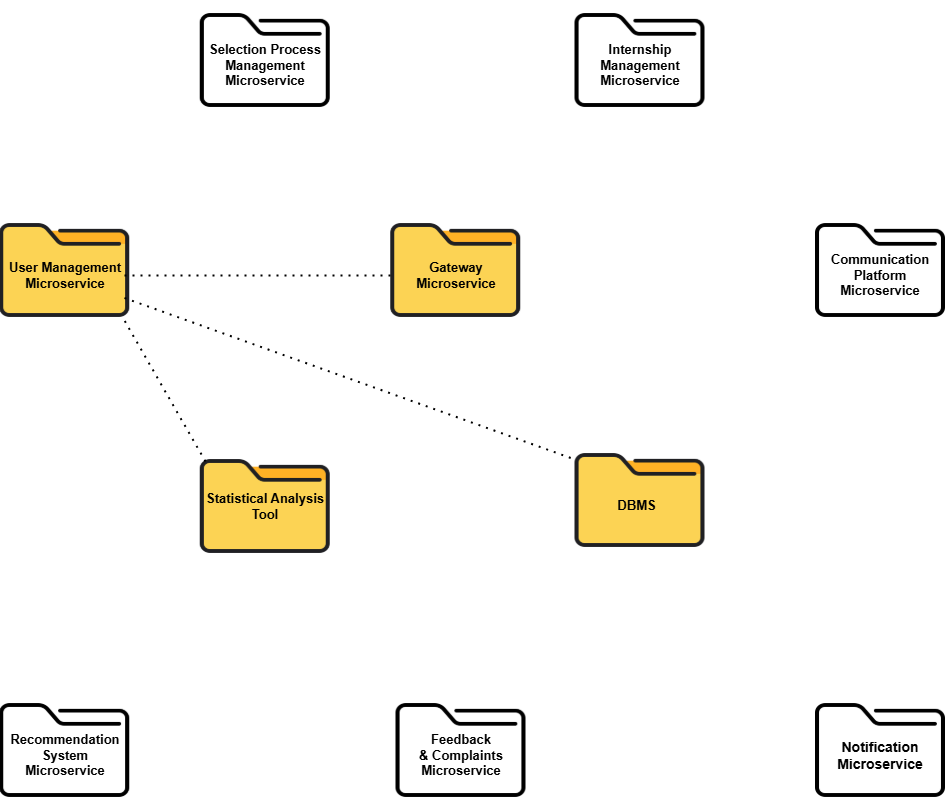
\includegraphics [width=0.75\linewidth] {test1.png}
\end{figure}

\subsubsection{Selection Process Management Features}

The selection process management feature is designed to guide both students and companies through
a series of steps ultimately culminating in the formal acceptance of the student for an internship.

The process begins when a student browses the available internship opportunities posted
by companies. This step is enabled by the gateway microservice, which provides the platform
interface and allows students to easily navigate through different company profiles and their
internship offers.
This step is made
possible also thanks to the usser management microservice that provides the
substance for this browsing process.
As the student explores these opportunities, their profile information,
preferences, and actions are managed by the student user management microservice, which ensures
their data is updated and stored in the database.

Once the student finds an internship that interests them, they can apply to start the selection
proess. This application triggers the selection process microservice, which records the
application and initiates the workflow for the company to review. The company can then
access the student's profile and decide whether to accept them into the selection process.
This decision-making is facilitated by the company user management microservice, which retrieves
the student's details stored in the database, allowing the company to make an informed decision
based on the student's qualifications and other relevant data.

If the company accepts the student, the notification microservice sends an automatic notification
to the student, informing them of the company's decision. This notification marks the official
start of the selection process, and the new association between the student and the company is
recorded in the system by the selection process microservice.

Once the student is accepted, the selection process continues with the student completing
questionnaires designed to assess their fit for the internship. These questionnaires are
managed and delivered by the selection process microservice, which ensures that they are
assigned to the appropriate students and tracked throughout the process. All responses
are stored in the database for later review by the company or other relevant stakeholders.

Additionally, the platform provides the option for online interviews, which can be scheduled
by the company and the student. The gateway microservice facilitates the scheduling and
conducting of these interviews, while the selection process microservice ensures that the
details of the interview, such as timing and participant information, are properly coordinated.
The user management microservices continue to handle the specific user data for both the student
and the company during this phase.
At the end if the selection process is successfully completed, the student is officially
accepted for the internship.

Finally, throughout the entire selection process, all information—including applications,
questionnaires, responses, and interview details—is stored in the database.
This centralized storage ensures that all data is easily accessible for future
reference, follow-ups, or reporting.

Here is a schematic view of the development and testing of this feature:

\begin{figure} [H]
    \centering
    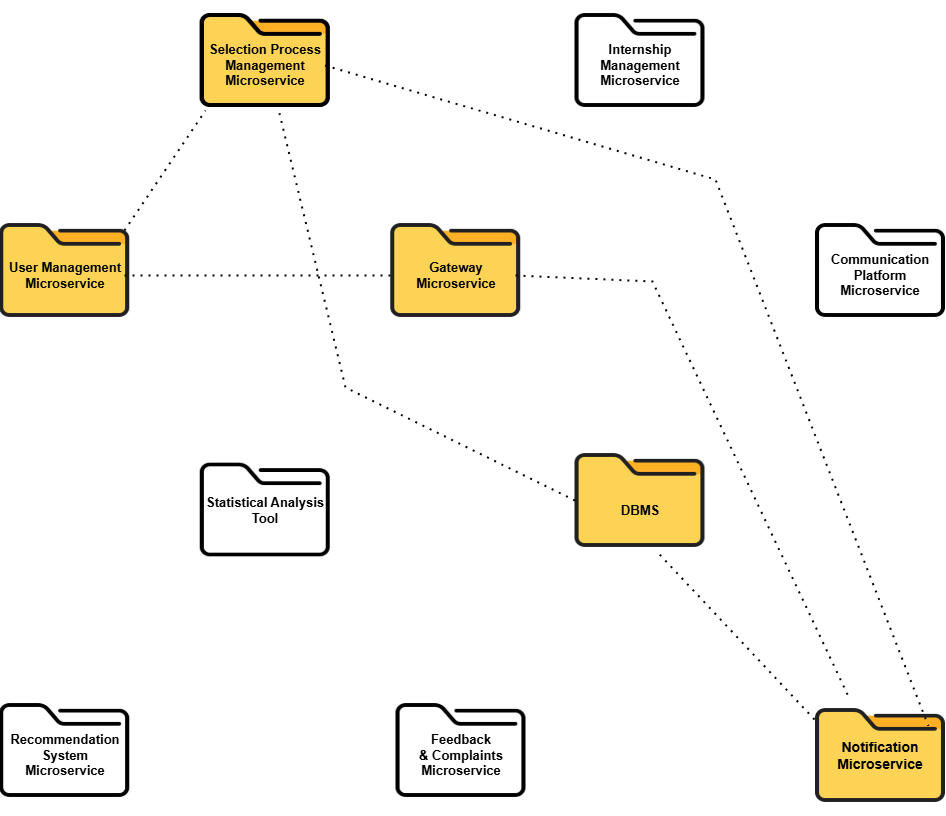
\includegraphics [width=0.75\linewidth] {test2.png}
\end{figure}

\subsubsection{Communication Features}

The communication feature is designed to enable effective interaction between students and
companies throughout the internship. The process begins when a user accesses the platform
through the gateway microservice, which handles user authentication and ensures secure
connections. After logging in, users can navigate to the relevant sections of the platform
where the communication tools are available.

One key component of this feature is the official internship page. This serves as a dedicated
space for interaction between students and companies, with distinct permissions assigned to
each party. Companies can use this page to post announcements related to the internship, and
students can engage with these posts by adding comments. The internship management microservice
ensures that announcements are correctly linked to their respective internship pages, while the
communication microservice facilitates the commenting functionality. To keep users informed, the
notification microservice sends alerts whenever new announcements are made.

Another important component is the direct chat system, which allows private communication between
students and companies. Messages exchanged through this chat are processed by the communication
microservice, ensuring secure and real-time delivery. Notifications for new chat messages are
generated by the notification microservice, ensuring that users are promptly alerted. All
interactions, including announcements, comments, and chat messages, are securely stored in
the database for future reference.

Notifications play a crucial role in this feature, ensuring that users are kept updated
about important events. Whether it’s a new announcement, a received message, or the conclusion
of an internship, the notification microservice manages the delivery of alerts. These notifications
are seamlessly integrated into the user experience via the gateway microservice, providing visibility
to users both during active sessions and upon logging in. Throughout the process, the internship
management microservice ensures that all communications and interactions are accurately associated
with their respective internships, with the database acting as the central repository for all related data.

Here is a schematic view of the development and testing of this feature:

\begin{figure} [H]
    \centering
    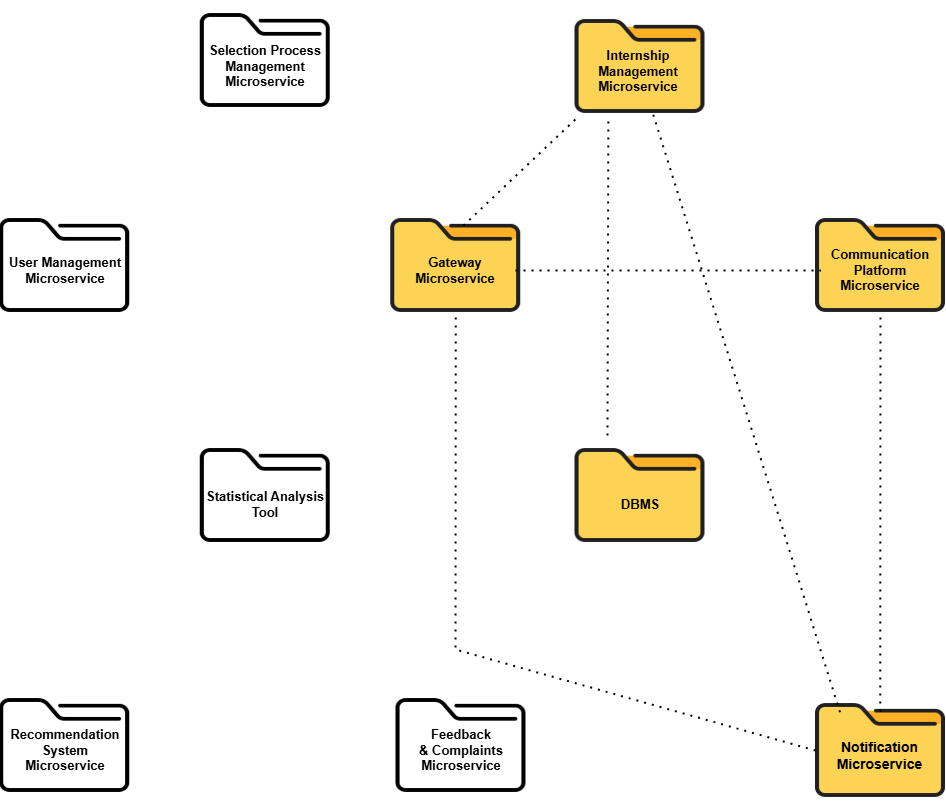
\includegraphics [width=0.75\linewidth] {test3.png}
\end{figure}

\subsubsection{Feedback and Complaints Collection Features}
\subsubsection{Providing Recommendations Features}
\subsubsection{Complaints Report Generation Features}


\newpage
\section{System Testing}

System testing is a critical phase of the development lifecycle where the fully
integrated Students \& Companies (S\&C) platform is rigorously evaluated to ensure that it
meets both functional and non-functional requirements. The testing environment is carefully
designed to closely replicate the actual production setup, enabling a comprehensive analysis
of the platform's behavior under realistic conditions.

Functional testing is focused on verifying that the platform meets the functional specifications
outlined in the requirements documentation, such as use cases. Key functionalities are examined,
including profile creation and management for both students and companies, the recommendation
system’s ability to match students with internships based on CV data and company requirements,
and support for the selection process, such as interview scheduling and structured questionnaires.
Communication features, including notifications and messaging, are tested to ensure seamless
interaction between users, while feedback and complaint management functionalities are validated
to confirm that users can effectively submit and track concerns.

Non-functional testing evaluates the system’s performance, scalability, and reliability under
a variety of conditions. This includes:

\begin{itemize}
\item Performance Testing: Measuring response times, throughput, and resource utilization to ensure that the
system operates efficiently under typical conditions.
\item Load Testing: Gradually increasing the number of concurrent users or sustaining a steady workload to
verify that the platform can handle expected user volumes without performance degradation.
\item Stress Testing: Simulating extreme conditions, such as sudden spikes in user activity or system failures,
to test the platform’s ability to recover and maintain availability in challenging scenarios.
\end{itemize}

To ensure thorough coverage, the testing methodology combines manual and automated approaches.
Manual testing is employed to validate specific scenarios, such as edge cases in the recommendation
system or workflows related to complaint resolution. Automated testing leverages techniques such as
fuzz testing, concolic execution, and search-based strategies, enabling repeated evaluations of the
system under varying conditions. These methods ensure the platform’s robustness, reliability, and
consistency across diverse environments.

Through this structured and comprehensive system testing approach, the S\&C platform is validated
to perform reliably and effectively in real-world scenarios, meeting the needs of students,
companies, and universities alike.